\documentclass{standalone}
\usepackage{tikz}
\usetikzlibrary{decorations.pathmorphing}
\usepackage{hsbcommon}
\begin{document}
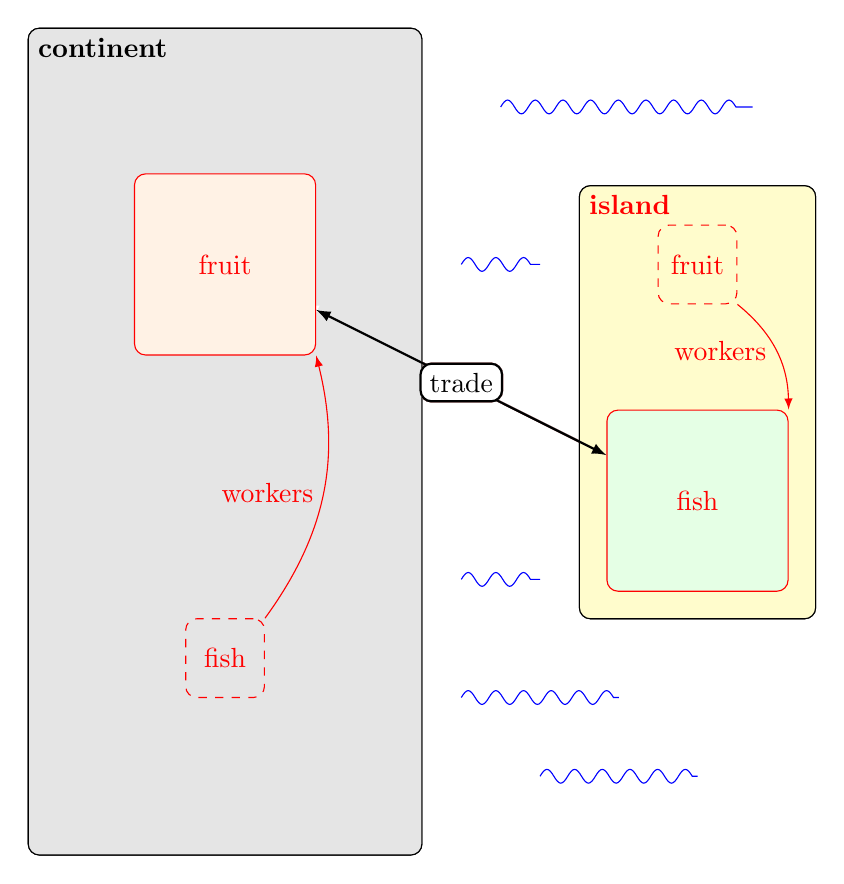
\begin{tikzpicture}
    \tikzset{
        fishernode/.style={draw, rounded corners, fill=green!10},
        planternode/.style={draw, rounded corners, fill=orange!10}
    }

    %% always: ocean squiggles
    \begin{scope}[color=blue]
        \draw[decorate,decoration={coil,aspect=0}] (-1.5,8) -- (1.7,8);
        \draw[decorate,decoration={coil,aspect=0}] (-2,6)   -- (-1,6);
        \draw[decorate,decoration={coil,aspect=0}] (-2,2)   -- (-1,2);
        \draw[decorate,decoration={coil,aspect=0}] (-2,0.5) -- (0,0.5);
        \draw[decorate,decoration={coil,aspect=0}] (-1,-0.5)-- (1,-0.5);
    \end{scope}

    %% always: continent + island, base nodes
    \draw[rounded corners, fill=gray!20]
        (-7.5,9) node[below right] {\textbf{continent}} rectangle (-2.5,-1.5);
    \node[fishernode,  minimum height=1cm, minimum width=1cm] (fl) at (-5,1) {fish};
    \node[planternode, minimum height=2cm, minimum width=2cm] (pl) at (-5,6) {fruit};
    \draw[<->,>=latex] (fl) -- node[draw,fill=white] {$4:1$} (pl);

    \begin{scope}[xshift=-4cm,yshift=2.5cm]
        \draw[rounded corners, fill=yellow!20]
            (3.5,4.5) node[below right] {\textbf{island}} rectangle (6.5,-1);
        \node[fishernode,  minimum height=2cm, minimum width=2cm] (fr) at (5,0.5) {fish};
        \node[planternode, minimum height=1cm, minimum width=1cm] (pr) at (5,3.5) {fruit};
        \draw[<->,>=latex] (fr) -- node[draw,fill=white] {$1:4$} (pr);
    \end{scope}

    %% step 2: trade arrow, mark nodes as out
    \ifstep{2}{
        \begin{scope}[color=red]
            \draw[<->,>=latex,thick] (fr) -- node[draw,rounded corners,fill=white] {trade} (pl);
            \node[fill=orange!10] at (pr) {(out)};
            \node[fill=green!10]  at (fl) {(out)};
        \end{scope}
    }

    %% step 3: erase old arrows with white, hide old labels
    \ifstep{3}{
        \begin{scope}[color=black]
            \draw[<->,>=latex,thick] (fr) -- node[draw,rounded corners,fill=white] {trade} (pl);
            \node[fill=orange!10] at (pr) {(out)};
            \draw[yellow!20,<->,>=latex] (fr) -- node[draw,fill=white] {$1:4$} (pr);
            \draw[yellow!20,<->,>=latex] (fl) -- node[draw,fill=white] {$1:4$} (pl);
        \end{scope}
        %% redraw continent + larger nodes showing specialisation
        \begin{scope}[color=red]
            \draw[rounded corners,color=black,fill=gray!20]
                (-7.5,9) node[below right] {\textbf{continent}} rectangle (-2.5,-1.5);
            \draw[<->,>=latex,thick,color=white] (fr) -- node[draw,rounded corners,fill=white] {trade} (pl);
            \begin{scope}
                \draw[<->,>=latex,color=gray!20] (fl) -- node[draw,color=gray!20,fill=gray!20] {$4:1$} (pl);
                \node[fishernode,dashed,fill=gray!20,minimum height=1cm,minimum width=1cm] (fl) at (-5,1) {fish};
                \node[planternode,minimum height=2.3cm,minimum width=2.3cm] (pl) at (-5,6) {fruit};
                \begin{scope}[xshift=-4cm,yshift=2.5cm]
                    \draw[rounded corners,fill=yellow!20,draw=black]
                        (3.5,4.5) node[below right] {\textbf{island}} rectangle (6.5,-1);
                    \node[fishernode,minimum height=2.3cm,minimum width=2.3cm] (fr) at (5,0.5) {fish};
                    \node[planternode,dashed,fill=yellow!20,minimum height=1cm,minimum width=1cm] (pr) at (5,3.5) {fruit};
                \end{scope}
                \draw[->,>=latex] (fl.north east) [bend right=25] to node[left] {workers} (pl.south east);
                \draw[<-,>=latex] (fr.north east) [bend right=25] to node[left] {workers} (pr.south east);
            \end{scope}
            \draw[<->,>=latex,thick,color=black] (fr) -- node[draw,rounded corners,fill=white] {trade} (pl);
        \end{scope}
    }

\end{tikzpicture}
\end{document}